\documentclass[serif,mathserif,final,table]{beamer}

\mode<presentation>{\usetheme{Lankton}}
\usepackage{graphicx}
\usepackage{gensymb}
\usepackage{adjustbox}
\usepackage{amsmath,amsfonts,amssymb,pxfonts,eulervm,xspace,bm,framed}
\usepackage[square,sort,comma,numbers]{natbib}
\bibliographystyle{apalike}
\usepackage[algo2e]{algorithm2e}
\usepackage{algorithmic}  
\usepackage{caption}
\usepackage{algorithm}
\DeclareCaptionFormat{myformat}{#3}
\captionsetup[algorithm]{format=myformat}
\algsetup{linenosize=\small}
\graphicspath{{./figures/}}
\usepackage[orientation=landscape,size=custom,width=90,height=60,debug]{beamerposter}


% Display a grid to help align images
%\beamertemplategridbackground[1cm]

%-- Header and footer information ----------------------------------
\newcommand{\footright}{\small Contact Email: bzk147@psu.edu}
\newcommand{\footleft}{\small }
\title{\Huge Dynamic Latent Factor Network Modeling (DLFM) \\ of the United Nations Voting Behaviors}
\author{Bomin Kim, Xiaoyue Niu, David Hunter, and Xun Cao}
\institute {Department of Statistics, Pennsylvania State University, State College, PA\\
	Department of Political Science, Pennsylvania State University, State College, PA}

%-------------------------------------------------------------------


%-- Main Document --------------------------------------------------

\begin{document}
	\nocite{*}
\begin{frame}{}
  \begin{columns}[t]

%-- Column 1 ----------------------------------------------------------
    \begin{column}{0.235\linewidth}
%%-- Block 1-1 -------------------------------------------------------
     \begin{block}{Abstract}
           	\begin{itemize}
           		\item Extension of additive-multiplicative latent factor model \cite{hoff2009multiplicative, hoff2014amen} to dynamic/longitudinal networks
                \item Adaptively estimate the Gaussian covariance structure to infer the temporal dependence
                \item Allowance of varying number of nodes over time
           	\end{itemize}
\begin{itemize}
           	\item  Our Findings:
            \begin{enumerate}
            \item DLFM is effective at predicting and explaining networks that are highly-correlated across timepoints
            \item DLFM acheives faster convergence and accuracy in parameter estimates, compared to the existing method
            \item DLFM's visualization of the results is useful to understand the temporal trends in networks
            \end{enumerate}
           	\end{itemize}
     
           \end{block}
%-- Block 1-1A
 	  \begin{block}{UN Voting Data}
 	  	
 	  	\begin{itemize}
 	  		\item Original dataset \cite{12379_2016} contains all roll-call votes in the United Nations General Assembly\\
 	  		\item Response variable $\boldsymbol{Y}$  \small{$(32 \times 23 \times 23 \mbox{ - dim. array})$}:
 	  		\begin{enumerate}
 	  		\item [-] Voting similarity index (0-1)
computed using 3 category vote data, only considering the important votes
\item [-] Years: from 1983 to 2014
\item [-] Nodes: 23 most active countries in 2004-2014
\begin{tabbing}
	\footnotesize
USA UKG FRN GMY RUS UKR GRG SUD IRN TUR IRQ EGY \\
	\footnotesize{SYR LEB ISR AFG CHN PRK ROK JPN IND PAK AUL}
\end{tabbing}
 	  		\end{enumerate}
 	  		\item Explanatory variables $\boldsymbol{X}$  \small{$(32 \times 23 \times 23 \times 5 \mbox{ - dim. array})$}:
 	  		\begin{enumerate}
             	\item Intercept: constant 1 (to estimate yearly baseline)
 	  			\item log($\mbox{distance}_{ij}$): log of the geographic distance between country $i$ and country $j$
 	  			\item $\mbox{Alliance}_{ijt}$: 1 if country $i$ and country $j$ have alliance in year $t$, and 0 otherwise
 	  			\item $\mbox{Polity score difference}_{ijt}$: absolute difference in polity IV number between country $i$ and country $j$, in year $t$
 	  			\item $\mbox{Relative trade}_{ijt}$: measure of relative importance of the trade between country $i$ and country $j$ in year $t$, using $$min\Big(\frac{\mbox{Trade}_{ijt}}{\mbox{GDP}_{it}}, \frac{\mbox{Trade}_{ijt}}{\mbox{GDP}_{jt}}\Big)$$
 	  		\end{enumerate}
 	  	\end{itemize}
 	            \end{block} 	
 	         
                	\begin{block}{References}
		{\tiny \bibliography{Ref} }
	\end{block}
    \end{column}
    
    
%-- Column 2 ---------------------------------------------------
    \begin{column}{0.235\linewidth}
           \begin{block}{Modeling Framework}
           	\begin{itemize}
           		\item For the symmetric matrices $\boldsymbol{Y}(t=1),...,\boldsymbol{Y}(t=T)$,
            \begin{equation*}
            \begin{aligned}
            &\boldsymbol{Y}_{N\times N}(t)=\sum_{p=1}^PX^p(t)\beta_p(t)+\Theta(t)+\Theta'(t)\\&\quad\quad\quad\quad+U(t)D(t)U'(t)+E(t), 
            \end{aligned}
            \end{equation*}
            where 
            \begin{enumerate}
            	\item[1.] $X(t)$ and $\beta(t)$: fixed effects from predictors
            	\item[2.] $\Theta(t)$ and $\Theta^\prime(t)$: additive row/column random effect
            	\item[3.] $U(t)D(t)U'(t)$: multiplicative random effect
            	\begin{tabbing}
            		- $U(t)$ is $N \times R$ matrix where $U_i(t) =(u_{i1}(t),...,u_{iR}(t))$ \\
            	- $D(t)$ is $R \times R$ matrix $(=\mbox{diag}(d_1(t),...,d_R(t)))$
            	\end{tabbing}
            	\item[4.] $E(t)$: random noise matrix
            \end{enumerate} 
            \vspace{10pt}
            \item Gaussian process (GP) prior specfication \cite{durante2014nonparametric}:
            \begin{enumerate}
         	\item[1.] For each covariate $p=1,...,P;$ $$\{\beta_{p}(t)\}_{t=1}^T\sim \mbox{MVN}_{T}(0, \tau^{\beta}_pc_\beta), \mbox{ with }\tau^{\beta}_p \sim \mbox{IG}(a_\beta, b_\beta)$$
         	\item[2.] For each node $i=1,...,N;$
         	$$\{\theta_{i}(t)\}_{t=1}^T \sim \mbox{MVN}_{T}(0, \tau^{\theta}_ic_\theta), \mbox{ with } \tau^{\theta}_i \sim \mbox{IG}(a_\theta, b_\theta)$$
         	\item[3.] For each dimension $r=1,...,R;$
         	 $$\{d_{r}(t)\}_{t=1}^T  \sim \mbox{MVN}_{T}(0, \tau^{d}_rc_d), \mbox{ with } \tau^{d}_r \sim \mbox{IG}(a_d, b_d)$$
         	\item[4.] For each node $i=1,...,N;$ and dimension $r=1,...,R;$ 
         	$$\{u_{ir}(t)\}_{t=1}^T \sim \mbox{MVN}_{T}(0, c_u)$$
         	\item[5.] For each pair of $(i, j)$ with $i > j,$
         	$$\epsilon_{ij}(t) \sim \mbox{N}(0, \sigma_e^2), \mbox{ with } \sigma_e^2 \sim \mbox{IG}(a, b),$$
            \end{enumerate}
            where $c_*$ is $T \times T$ correlation matrix corresponding to $* \in \{\beta, \theta, d, u\}$ obtained from the GP function 
            \begin{equation*}
c_*(t, t')=\begin{cases}
\mbox{exp}(-\frac{|t-t'|}{\kappa_*}), & \mbox{covfc = Exponential}\\
\mbox{exp}(-\frac{||t-t'||_2^2}{\kappa_*^2}), & \mbox{covfc = Sq. Exponential}\\
\end{cases}
            \end{equation*}
            Note: each value of $\kappa_*$ and the corresponding proper covariance function is estimated. 
                        \vspace{10pt}
                        \item Bayesian Inference using Gibbs sampling (MCMC):\\
                        Sequentially resample each of latent variables
                        \begin{equation*}
                        \begin{aligned}
                      	&\Big(\sigma_e^2, \{\tau^{\beta}_p\}_{p=1}^P, \{\tau^{\theta}_i\}_{i=1}^N, \{\tau^{d}_r\}_{r=1}^R, \{\{\beta_{p}(t)\}_{t=1}^T\}_{p=1}^P, \\& \{\{\theta_{i}(t)\}_{t=1}^T\}_{i=1}^N, \{\{d_{r}(t)\}_{t=1}^T \}_{r=1}^R, \{\{\{u_{ir}(t)\}_{t=1}^T\}_{i=1}^N\}_{r=1}^R\}\Big)
                        \end{aligned}                        
\end{equation*}
                        from the full conditional distributions
        \end{itemize}
            \end{block}
     

      %-- Block 2-2
    \end{column}
    %2

    %-- Column 3 ---------------------------------------------------
    \begin{column}{0.235\linewidth}
    	
    	      %-- Block 2-2
    	      \begin{block}{Adaptive sampling algorithm}
    	       		 \begin{algorithm}[H]
    	       		 	\SetAlgoLined
    	       		 	\caption{\textcolor{darkblue}{1. }\textbf{Scanning with temporal independence}}
    	       		\For{\mbox{iter}=1 to \mbox{scan}}{
    	       				run MCMC with $\boldsymbol{ \kappa}_* =0.001$ (which gives $c_* = I_T$)
    	       			}
    	       			\end{algorithm}
    	       		   	 \begin{algorithm}[H]
    	       		   	 	\caption{\textcolor{darkblue}{2. }\textbf{Estimating covariance structure}}
    	       		   	 	\For {$*$ in $(\beta, \theta, d, u)$}{
    	       		   	 calculate the correlation $\rho_{t,t'}^*$ and compare the fittings\\
    	       		   	-  Exponential: $\mbox{log}(\rho_{t,t'}^*) =-\frac{1}{\kappa}|t-t^\prime|$\\
    	       		   	- Sq. Exponential: $\mbox{log}(\rho_{t,t'}^*)= -\frac{1}{\kappa^2}||t-t^\prime||_2^2$\\
    	       		   	 construct $\hat c_*$ given $\hat{\kappa}_*$ and covfc with better fit}
    	       		   	\end{algorithm}
    	       		   	 \centering
    	       		   	 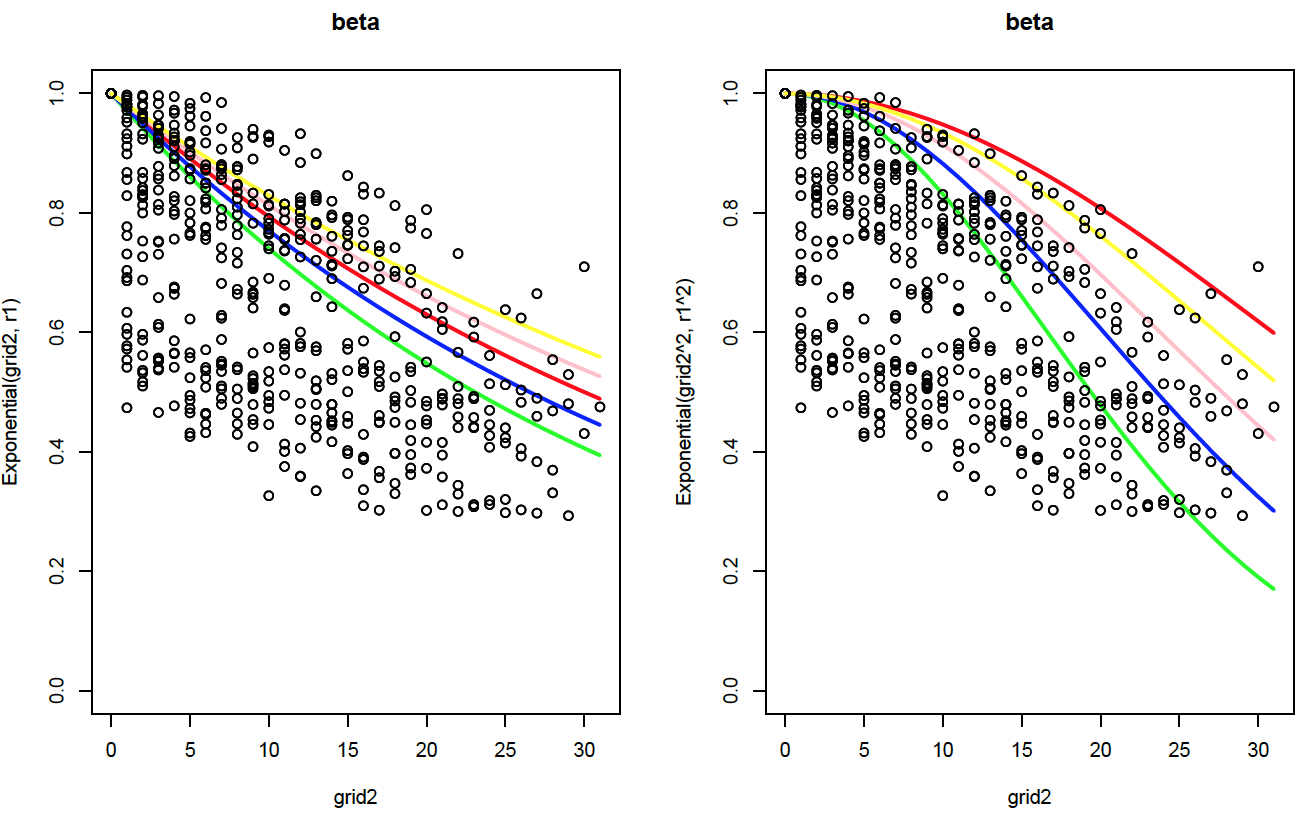
\includegraphics[width=0.67\textwidth]{betacor.jpeg}
    	       		    \begin{algorithm}[H]
    	       		    	\caption{\textcolor{darkblue}{3. }\textbf{Running with temporal dependence}}
    	       		   	\For{\mbox{iter}=1 to nsample}{
    	       		   		run MCMC with estimated $\hat c_* = (\hat c_\beta, \hat c_\theta,\hat c_d, \hat c_u)$
    	       		   	}
    	       		   	Summarize the results only using the new samples with estimated temporal dependence structure
    	       		   \end{algorithm}    	       		  
    	      \end{block}
    	      
    
		\begin{block}{Varying number of nodes}
		\begin{itemize}
		\item New node can join or existing node can disappear at any timepoint\\
		\small (ex. countries not existed: RUS $\sim$1988, UKR $\sim$1986, GRG $\sim$1989; countries in war: IRQ 1995-2003)
		\normalsize  
		\item Allow ``structural NA's" remain as NA, while pure missing values imputed using posterior estimates
        \begin{enumerate}
        \item Reduce bias in fixed effect estimates $\beta$
        \item Avoid meaningless random effect estimates $\Theta$ and $U$
        \item Provide flexibility in fitting the model to larger networks (limitation: with known in-and-out structure)
        \end{enumerate}
		\end{itemize}
					\end{block}
      	\end{column}
%-- Column 4 ---------------------------------------------------     	 
\begin{column}{0.235\linewidth}  
	\begin{block}{Results}

		\begin{itemize}
            \item Fixed effect estimates $\beta$	\end{itemize}
             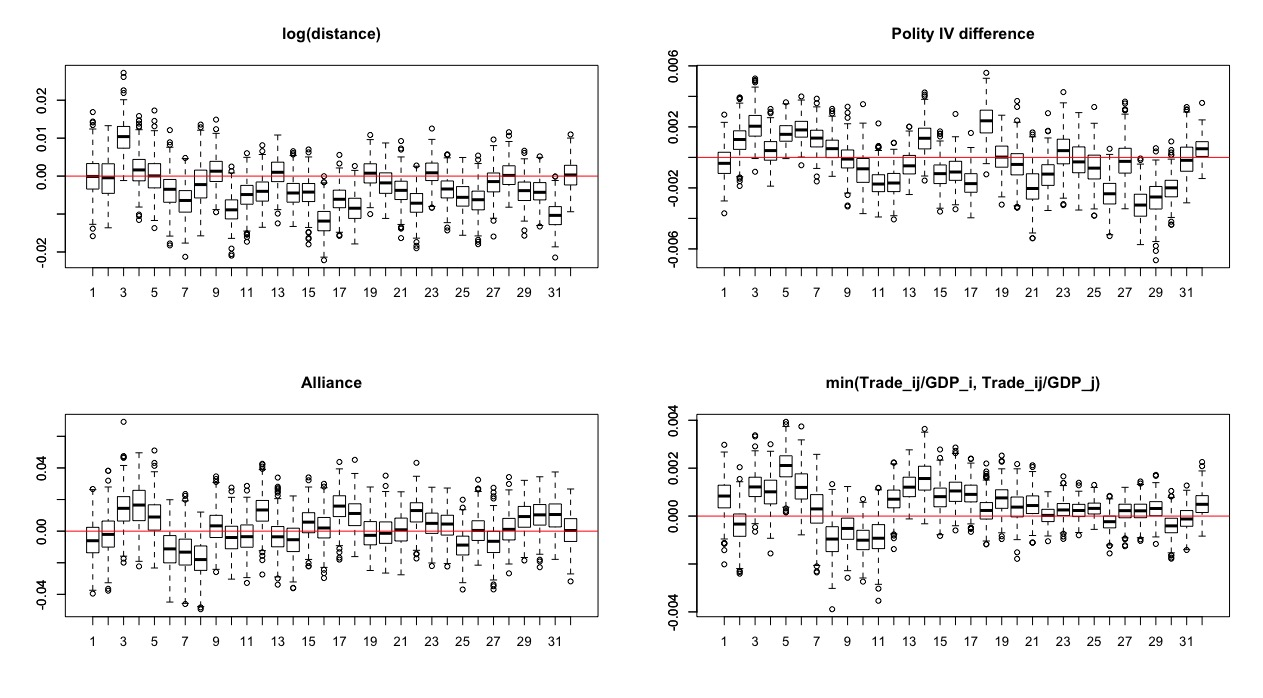
\includegraphics[width=0.967\textwidth]{betaplot.jpeg}		\begin{itemize}
            \item Additive random effect estimates $\Theta$	\end{itemize}
             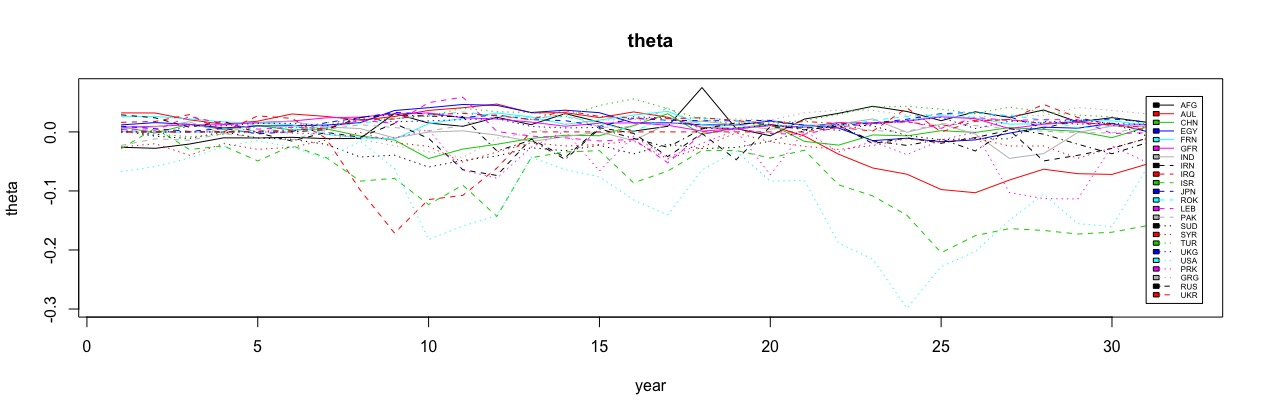
\includegraphics[width=0.967\textwidth]{thetaplot.jpeg}		\begin{itemize}
            \item Multiplicative random effect estimates $U$ and $D$
            		\end{itemize}
               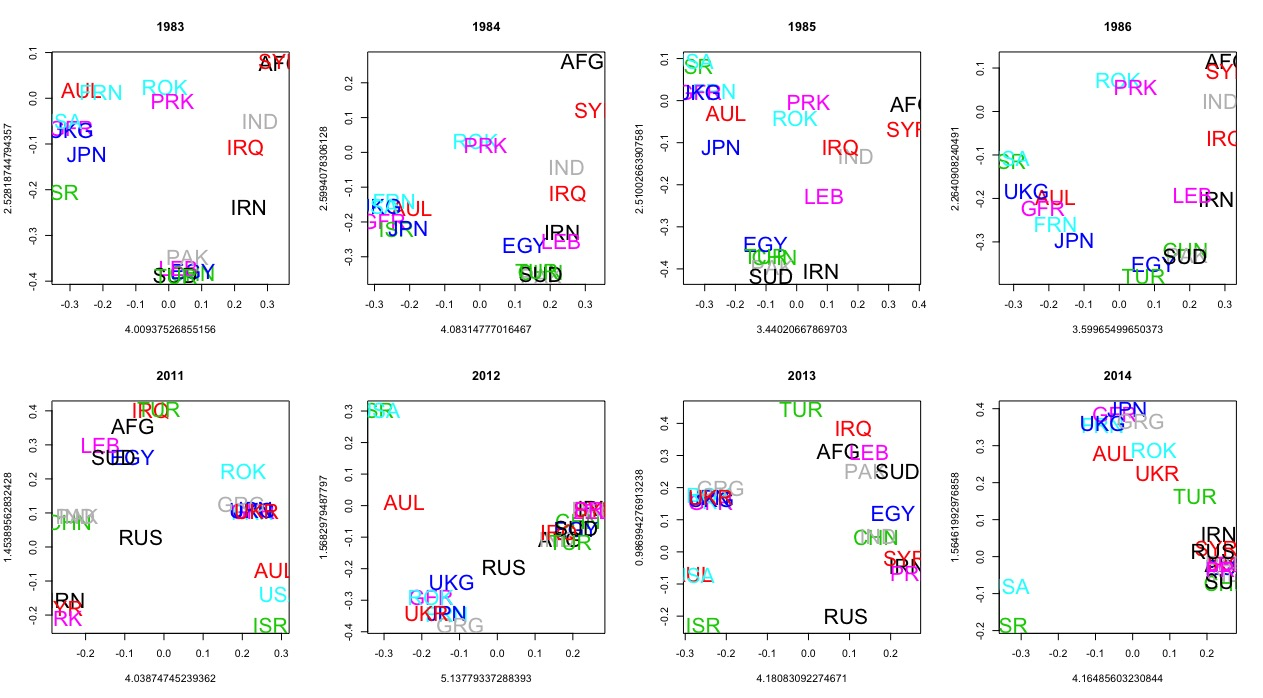
\includegraphics[width=0.967\textwidth]{UDUplot.jpeg}


	\end{block}
	
	\begin{block}{Conclusions}
		\begin{enumerate}
\item DLFM estimates of fixed effects and random effects show interesting foreign policy trends in UN voting behaviors, revealing noticeable difference in the Cold War era and post-Cold War era
\item Computationally outperform the multiple fittings of static model (R package `AMEN' \cite{hoff2014amen})
			\end{enumerate}
	\end{block}
	

\end{column}
  \end{columns}
\end{frame}
\end{document}
